\documentclass[10pt,pdf,hyperref={unicode}]{beamer}

\mode<presentation>
{
\usetheme{boxes}
\beamertemplatenavigationsymbolsempty

\setbeamertemplate{footline}[page number]
\setbeamersize{text margin left=1em, text margin right=0.5em}
}

\usepackage[utf8]{inputenc}
\usepackage[english, russian]{babel}
\usepackage[normalem]{ulem}
\usepackage{bm}
\usepackage{multirow}
\usepackage{ragged2e}
\usepackage{indentfirst}
\usepackage{multicol}
\usepackage{subfig}
\usepackage{amsmath,amssymb}
\usepackage{dsfont}
\usepackage{enumerate}
\usepackage{mathtools}
\usepackage{comment}
\usepackage{multicol}
\usepackage[all]{xy}

\newcommand{\bz}{\mathbf{z}}
\newcommand{\bx}{\mathbf{x}}
\newcommand{\by}{\mathbf{y}}
\newcommand{\bv}{\mathbf{v}}
\newcommand{\bw}{\mathbf{w}}
\newcommand{\ba}{\mathbf{a}}
\newcommand{\bb}{\mathbf{b}}
\newcommand{\bff}{\mathbf{f}}
\newcommand{\bh}{\mathbf{h}}
\newcommand{\bl}{\mathbf{l}}
\newcommand{\bp}{\mathbf{p}}
\newcommand{\bq}{\mathbf{q}}
\newcommand{\bs}{\mathbf{s}}
\newcommand{\bt}{\mathbf{t}}
\newcommand{\bu}{\mathbf{u}}
\newcommand{\bT}{\mathbf{T}}
\newcommand{\bX}{\mathbf{X}}
\newcommand{\bZ}{\mathbf{Z}}
\newcommand{\bS}{\mathbf{S}}
\newcommand{\bH}{\mathbf{H}}
\newcommand{\bW}{\mathbf{W}}
\newcommand{\bY}{\mathbf{Y}}
\newcommand{\bU}{\mathbf{U}}
\newcommand{\bQ}{\mathbf{Q}}
\newcommand{\bP}{\mathbf{P}}
\newcommand{\bA}{\mathbf{A}}
\newcommand{\bB}{\mathbf{B}}
\newcommand{\bC}{\mathbf{C}}
\newcommand{\bE}{\mathbf{E}}
\newcommand{\bF}{\mathbf{F}}
\newcommand{\bsigma}{\boldsymbol{\sigma}}
\newcommand{\bomega}{\boldsymbol{\omega}}
\newcommand{\btheta}{\boldsymbol{\theta}}
\newcommand{\bgamma}{\boldsymbol{\gamma}}
\newcommand{\bdelta}{\boldsymbol{\delta}}
\newcommand{\bPsi}{\boldsymbol{\Psi}}
\newcommand{\bpsi}{\boldsymbol{\psi}}
\newcommand{\bxi}{\boldsymbol{\xi}}
\newcommand{\bmu}{\boldsymbol{\mu}}
\newcommand{\bchi}{\boldsymbol{\chi}}
\newcommand{\bzeta}{\boldsymbol{\zeta}}
\newcommand{\blambda}{\boldsymbol{\lambda}}
\newcommand{\beps}{\boldsymbol{\varepsilon}}
\newcommand{\bZeta}{\boldsymbol{Z}}
% mathcal
\newcommand{\cX}{\mathcal{X}}
\newcommand{\cY}{\mathcal{Y}}
\newcommand{\cW}{\mathcal{W}}

\newcommand{\dH}{\mathds{H}}
\newcommand{\dR}{\mathds{R}}
% transpose
\newcommand{\T}{^{\mathsf{T}}}

% command to strike out text
\newcommand{\stkout}[1]{\ifmmode\text{\sout{\ensuremath{#1}}}\else\sout{#1}\fi}

\renewcommand{\epsilon}{\ensuremath{\varepsilon}}
\renewcommand{\phi}{\ensuremath{\varphi}}
\renewcommand{\kappa}{\ensuremath{\varkappa}}
\renewcommand{\le}{\ensuremath{\leqslant}}
\renewcommand{\leq}{\ensuremath{\leqslant}}
\renewcommand{\ge}{\ensuremath{\geqslant}}
\renewcommand{\geq}{\ensuremath{\geqslant}}
\renewcommand{\emptyset}{\varnothing}

\usepackage{tikz}
\usetikzlibrary{positioning,arrows}

\tikzstyle{name} = [parameters]
\definecolor{name}{rgb}{0.5,0.5,0.5}

\usepackage{caption}
\captionsetup{skip=0pt,belowskip=0pt}

\newtheorem{rustheorem}{Теорема}
\newtheorem{russtatement}{Утверждение}
\newtheorem{rusdefinition}{Определение}

% colors
\definecolor{darkgreen}{rgb}{0.0, 0.2, 0.13}
\definecolor{darkcyan}{rgb}{0.0, 0.55, 0.55}

\AtBeginEnvironment{figure}{\setcounter{subfigure}{0}}

\captionsetup[subfloat]{labelformat=empty}
\addto\captionsrussian{\renewcommand{\figurename}{}}
\graphicspath{{../figures/}}

%----------------------------------------------------------------------------------------------------------

\title[Заголовок]{Выбор моделей пространства состояний в задаче нейронного декодирования}
\author{Владимиров Э.А.}

\institute[]{Московский физико-технический институт}
\date{\footnotesize
	\par\smallskip\emph{Эксперт:} В.\,В.~Стрижов
	\par\smallskip\emph{Консультант:} А.\,М.~Самохина
	\par\bigskip\small 2023}

%---------------------------------------------------------------------------------------------------------
\begin{document}

\begin{frame}
\titlepage
\end{frame}

%----------------------------------------------------------------------------------------------------------
\begin{frame}{Нейронное декодирование}
	\begin{alertblock}{Проблема}
		Агрегирование информации во времени
	\end{alertblock}
	
	\begin{alertblock}{Задача}
		Выбор модели пространства состояний
	\end{alertblock}
	
	\begin{alertblock}{Решение}
		Сделать выбор на основе анализа свойств моделей
	\end{alertblock}
\end{frame}

%---------------------------------------------------------------------------------------------------------
\begin{frame}{Модель пространства состояний}
	\begin{multicols}{2}
		\begin{gather*}
			\text{Непрерывная модель пр-ва состояний} \\
			x'(t) = Ax(t) + Bu(t) \\
			y(t) = Cx(t) + \stkout{Du(t)} \\ \\
			\text{Дискретная модель пр-ва состояний} \\
			x_k = Ax_{k-1} + Bu_k \\
			y_k = Cx_k + \stkout{Du_k}
		\end{gather*}
	
		\begin{gather*}
		\end{gather*}
	
		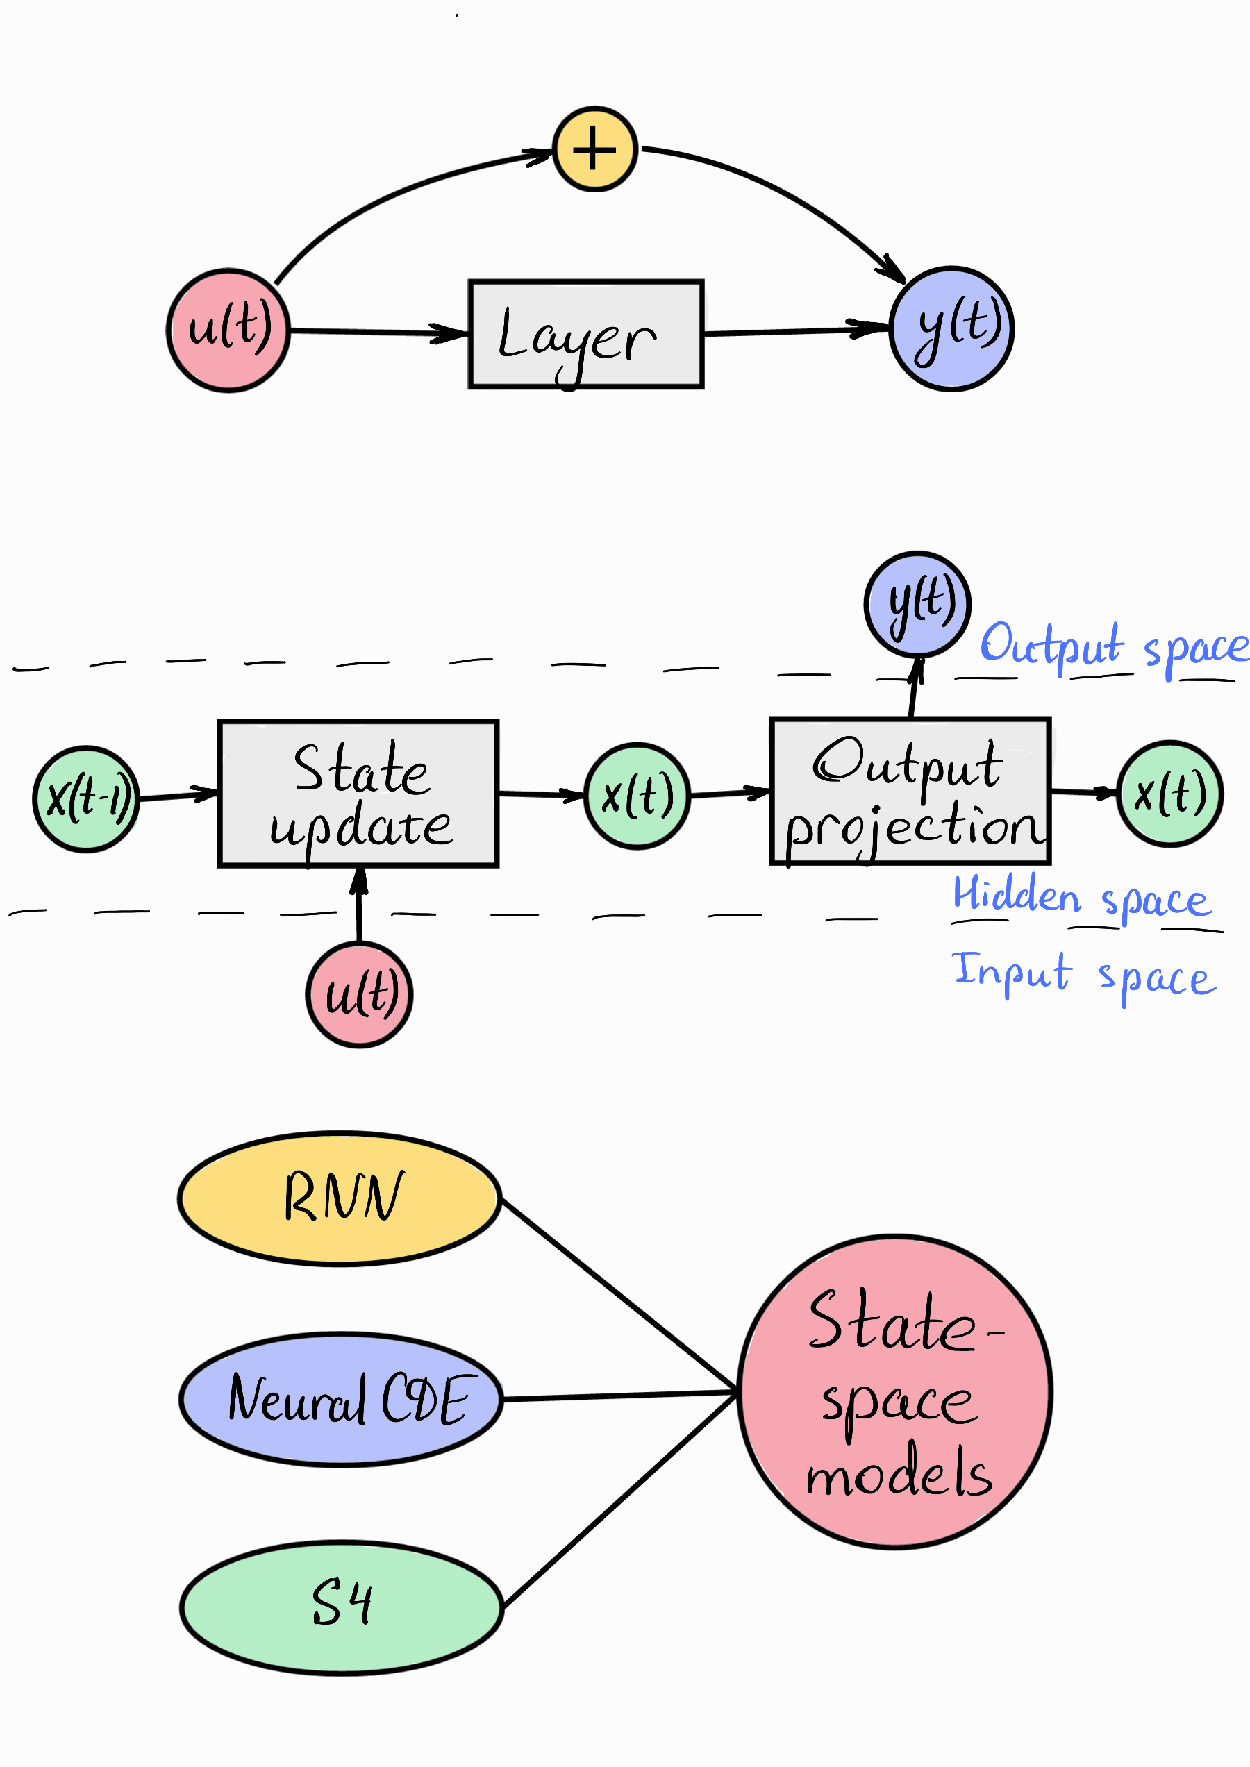
\includegraphics[width=0.45\textwidth]{3rd-slide.pdf}
	\end{multicols}
\end{frame}

%--------------------------------------------------------------------------------------------------------
%\begin{frame}{История моделей}
%	\begin{figure}
%		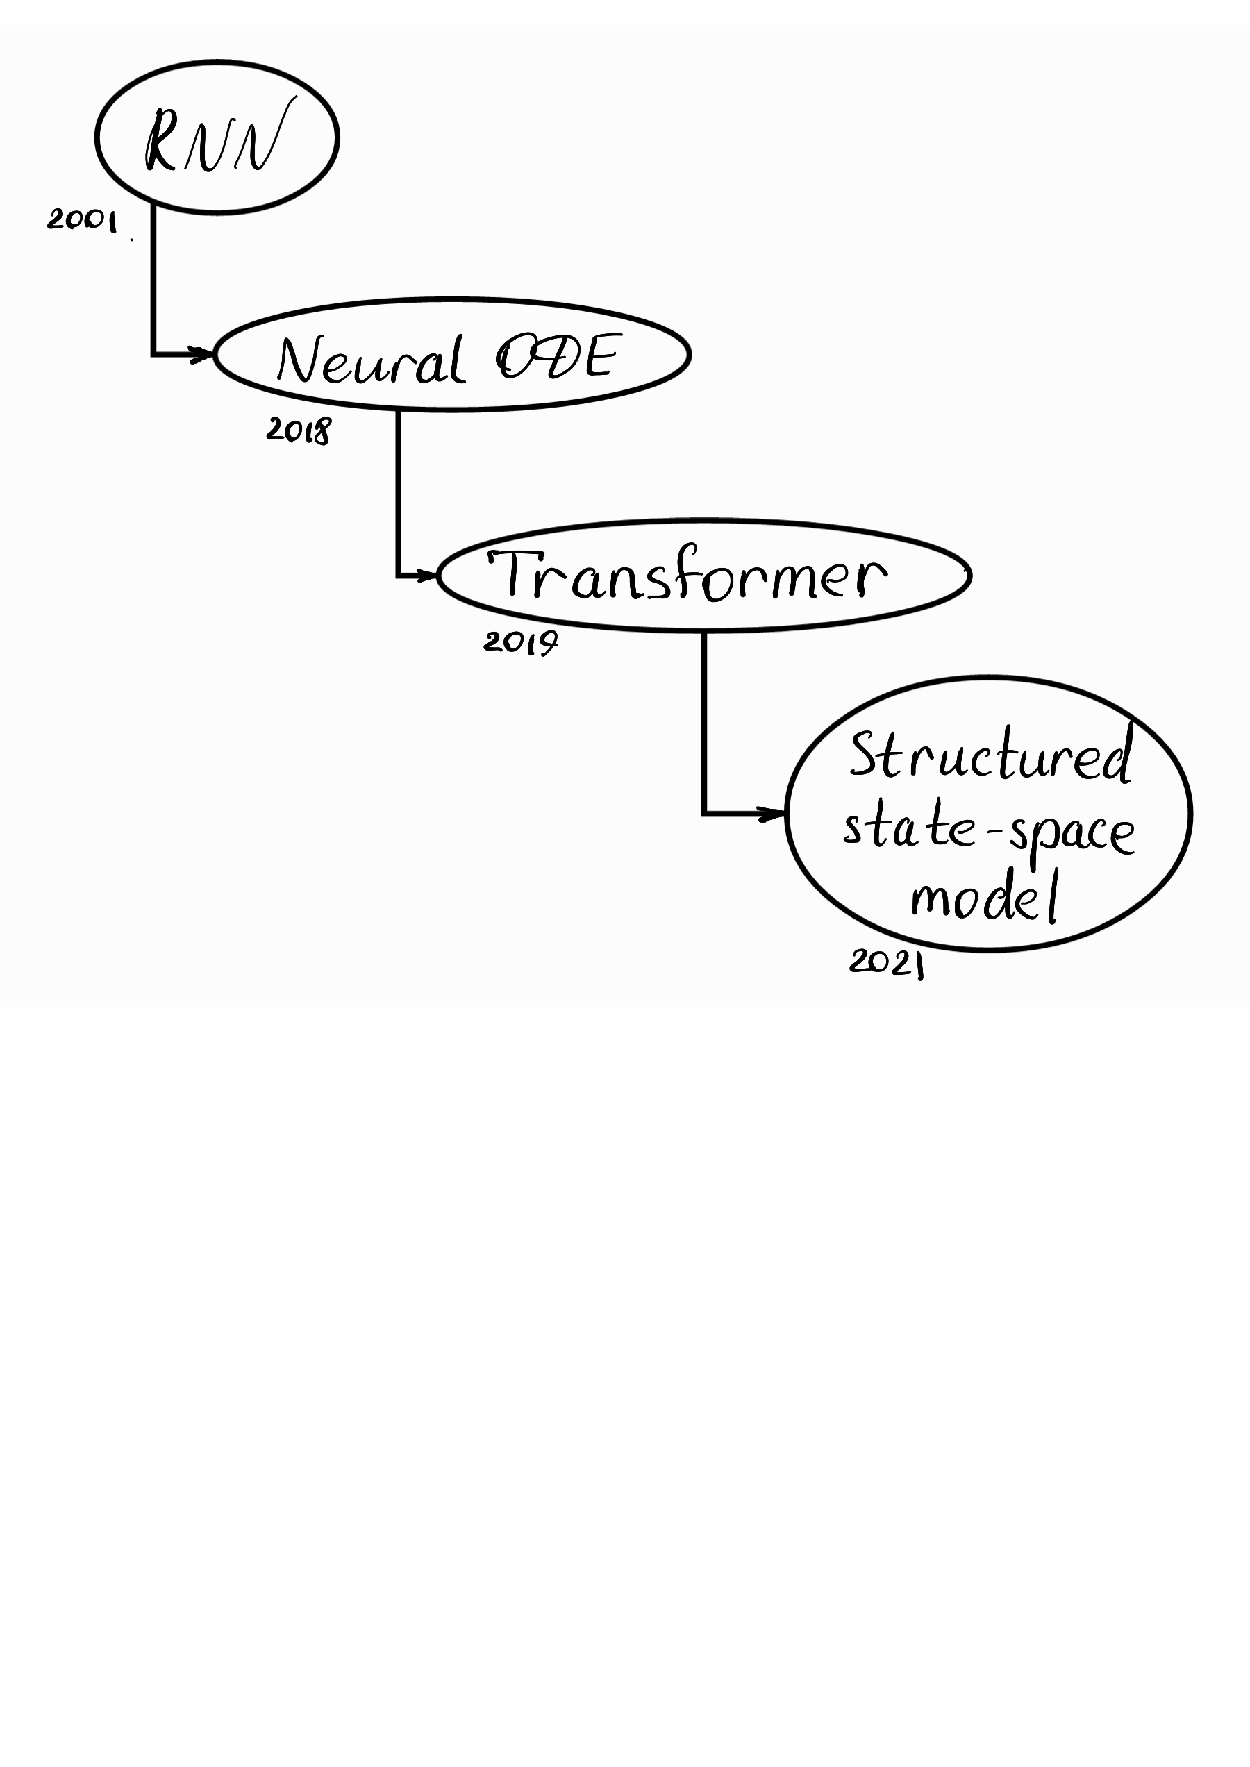
\includegraphics[width=0.85\textwidth]{ts-models-history.pdf}
%	\end{figuree
%\end{frame}

\begin{frame}{Нейронное декодирование}
	$\bX \in \dR^{M \times N \times T}$ ~--- $M$ измерений ЭКГ, где $N$ ~--- число электродов, $T$ ~--- число элементов временного ряда
	
	$Y \in \{ 0, 1\}^M$ ~--- целевая переменная
	
	Критерий качества ~--- бинарная кросс-энтропия  
	
	$$ L(\bw) = -\dfrac{1}{M} \sum\limits_{m=1}^M y_m \log(f(\bw, \bx)) + (1 - y_m) \log(1 - f(\bw, \bx))$$
	
	Оптимизационная задача: $\hat{\bw} = \underset{\bw}{\arg \max} L(\bw)$
\end{frame}

%---------------------------------------------------------------------------------------------------------
\begin{frame}{Рекуррентные нейронные сети}
	\begin{multicols}{2}
		\begin{figure}
			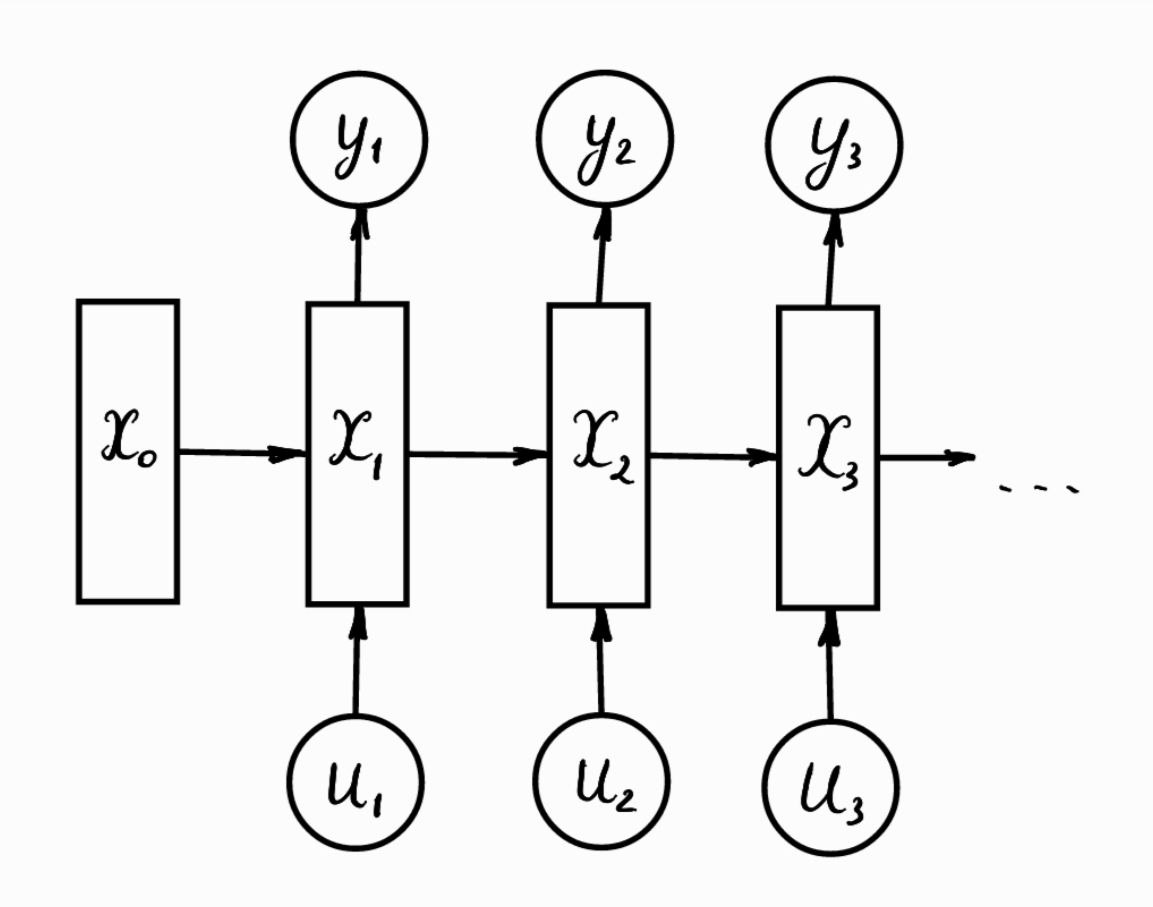
\includegraphics[width=0.5\textwidth]{rnn.jpg}
		\end{figure}
		
		\begin{equation*}
			\mbox{\Large\(
				\begin{aligned}
					\bx_t &= \sigma_x(W_x \bx_{t-1} + W_u \bu_t) \\
					\by_t &= \sigma_y(W_y \bx_t),
				\end{aligned}
			\)}
		\end{equation*}
		$\text{где } \bu_i \in \dR^d, \; \bx_i \in \dR^K \; \by_i \in \dR^s$  
		
		$\sigma: \dR^K \rightarrow \dR^K$ ~--- функция активации  
		
		$W_x \in \dR^{K \times K}, W_u \in \dR^{s \times K}, W_y \in \dR^{K \times d}$ ~--- матрицы весов
	\end{multicols}
	\bigskip
	\footnotetext[1]{\textit{Medsker L. R., Jain L. C.} Recurrent neural networks //Design and Applications. – 2001. – Т. 5. – С. 64-67.}
\end{frame}
%----------------------------------------------------------------------------------------------------------
\begin{frame}{Сравнение РНС с моделью пространства состояний}
	\begin{multicols}{2}
		\mbox{\Large\(
			\begin{aligned}
				&\text{\normalsize{Модель пространства состояний}} \\
				&\bx_t = A\bx_{t-1} + B\bu_t \\
				&\by_t = C\bx_{t}
			\end{aligned}
		\)}

		\mbox{\Large\(
			\begin{aligned}
				&\text{\normalsize{Рекуррентная нейронная сеть}} \\
				&\bx_t = \sigma(W_x \bx_{t-1} + W_u \bu_t) \\
				&\by_t = W_y \bx_t
			\end{aligned}
		\)}
	\end{multicols}
\end{frame}

%----------------------------------------------------------------------------------------------------------
\begin{frame}{Нейронные контролируемые дифференциальные уравнения}
	\begin{multicols}{2}
		\begin{figure}
			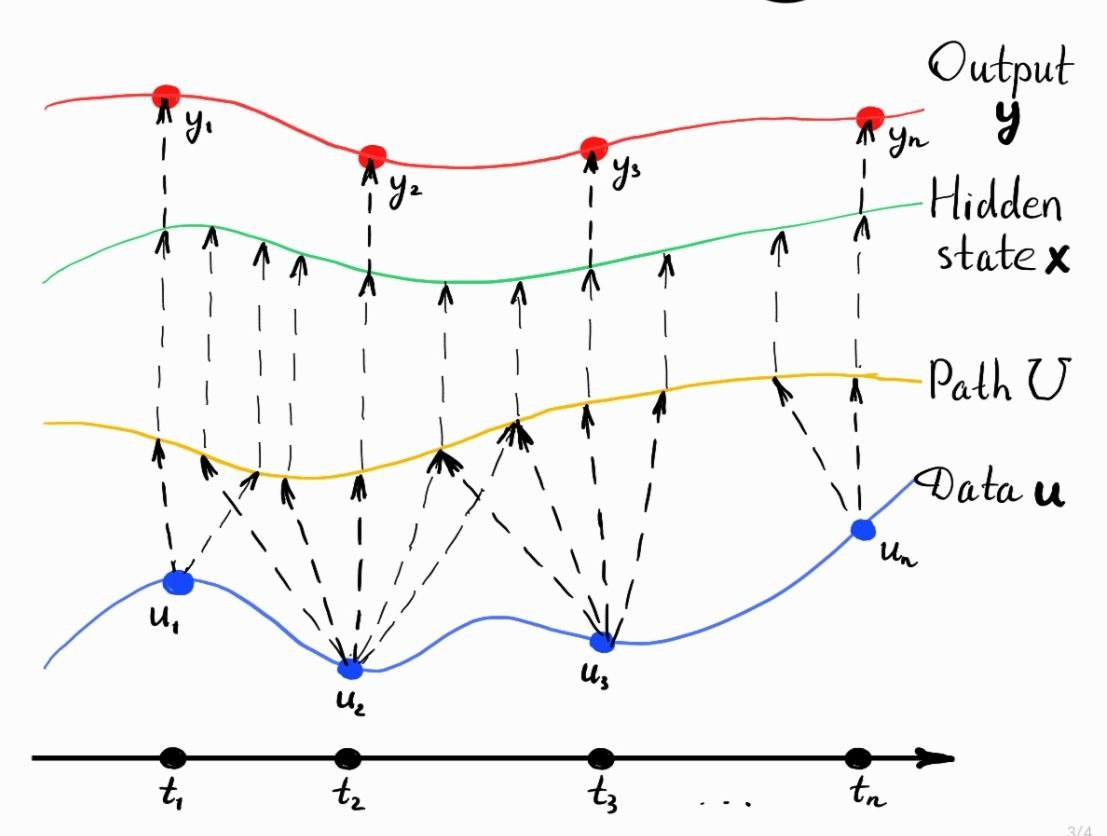
\includegraphics[width=0.5\textwidth]{neural-cde-path.jpg}
		\end{figure}
	
		\begin{equation*}
			\begin{cases}
				\bx(t_1) = \zeta(\bu_1, t_1) \\
				\bx(t) = \bx(t_1) + \int_{t_1}^t \bff(\bx(\tau))dU(\tau) \\
				\by_i = g(\bx(t_i))
			\end{cases}
		\end{equation*}
		$\text{где } \bu_i \in \dR^d, \; \by_i \in \dR^s $
		
		$\bx: [t_1, t_n] \rightarrow \dR^K$ ~--- функция скрытого состояния
		
		$U: [t_1, t_n] \rightarrow \dR^{d+1}$ ~--- кубический сплайн 
		
		$\zeta: \dR^{d+1} \rightarrow \dR^K$ ~--- проектор в скрытое пространство
		
		$f: \dR^K \rightarrow \dR^{K \times (d+1)}$ ~--- динамика скрытого состояния
		
		$g: \dR^K \rightarrow \dR^s$ ~--- линейное отображение
	\end{multicols}
\end{frame}

%----------------------------------------------------------------------------------------------------------
\begin{frame}{Сравнение НКДУ с моделью пространства состояний}
	\begin{multicols}{2}
		\mbox{\Large\(
			\begin{aligned}
				&\text{\normalsize{Модель пространства состояний}} \\
				&\bx(t_1) = Const \\
				&\bx'(t) = A\bx(t) + B\bu(t) \\
				&\by(t) = C\bx(t)
			\end{aligned}
		\)}
		
		\mbox{\Large\(
			\begin{aligned}
				&\text{\normalsize{Нейронные КДУ}} \\
				&\bx(t_1) = A\bu(t_1) + f(t_1) \\
				&\bx'(t) = BU'(t) \cdot \bx(t) \\
				&\by(t) = C \bx(t)
			\end{aligned}
		\)}
	\end{multicols}
	\bigskip
	\footnotetext[1]{\textit{Kidger P. et al.} Neural controlled differential equations for irregular time series //Advances in Neural Information Processing Systems. – 2020. – Т. 33. – С. 6696-6707}
\end{frame}

%----------------------------------------------------------------------------------------------------------
\begin{frame}{Модели структурированного пространства состояний}
	\begin{figure}
		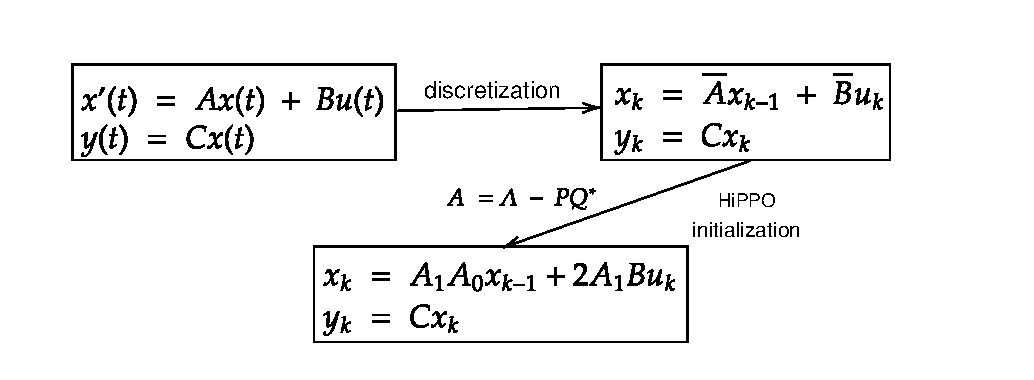
\includegraphics[width=0.9\textwidth]{s4-diagram.pdf}
	\end{figure}

	\begin{multicols}{2}
		\begin{align*}
			&u_k = u(k\Delta) \\
			&\overline{A} = (I - \dfrac{\Delta}{2} A)^{-1} (I + \dfrac{\Delta}{2} A) \\
			&\overline{B} = (I - \dfrac{\Delta}{2} A)^{-1} \Delta B
		\end{align*}
	
		\begin{align*}
			&A = \Lambda - PQ^* \text{~--- диаг. + ранг 1}\\
			&A_0 = \dfrac{2}{\Delta} I + A \\
			&D = (\dfrac{2}{\Delta} - \Lambda)^{-1} \\
			&A_1 = D - DP(1 + Q^*DP)^{-1}Q^*D
		\end{align*}
	\end{multicols}
	\footnotetext[1]{\textit{Gu, Albert, Karan Goel, and Christopher Ré} Efficiently modeling long sequences with structured state spaces //arXiv preprint arXiv:2111.00396. – 2021}
\end{frame}
%----------------------------------------------------------------------------------------------------------
\begin{frame}{Итоговое сравнение моделей}
	$L$ ~--- длина последовательности
	
	$d$ ~--- размерность исходного пространства
	
	$K$ ~--- размерность скрытого пространства
	
	$s$ ~--- размерность целевого пространства
	
	$M = \max(d, K, s)$  
	
	\begin{table}
		\begin{tabular}{c|l|l|}
			\cline{2-3}
			\multicolumn{1}{l|}{}             & Parameters & Forward \\ \hline
			\multicolumn{1}{|c|}{RNN}         & $O(KM)$ & $O(KML)$ \\ \hline
			%\multicolumn{1}{|c|}{Transformer} & $O(K^2d + Ks)$ & $O(LK \cdot (L+S))$ \\ \hline
			\multicolumn{1}{|c|}{Neural CDE}  & $O(K^2d + Ks)$ & $O(K^2dL)$ \\ \hline
			\multicolumn{1}{|c|}{S4}          & $O(Kd + Ks)$ & $O(KML)$ \\ \hline
		\end{tabular}
	\end{table}
\end{frame}
%----------------------------------------------------------------------------------------------------------
\begin{frame}{Вычислительный эксперимент}
	\begin{alertblock}{Цель}
		 На примере задачи классификации сигналов ЭКГ сравнить работу различных моделей пространства состояний
	\end{alertblock}

	Основная модель ~--- HTNet
	
	\begin{figure}
		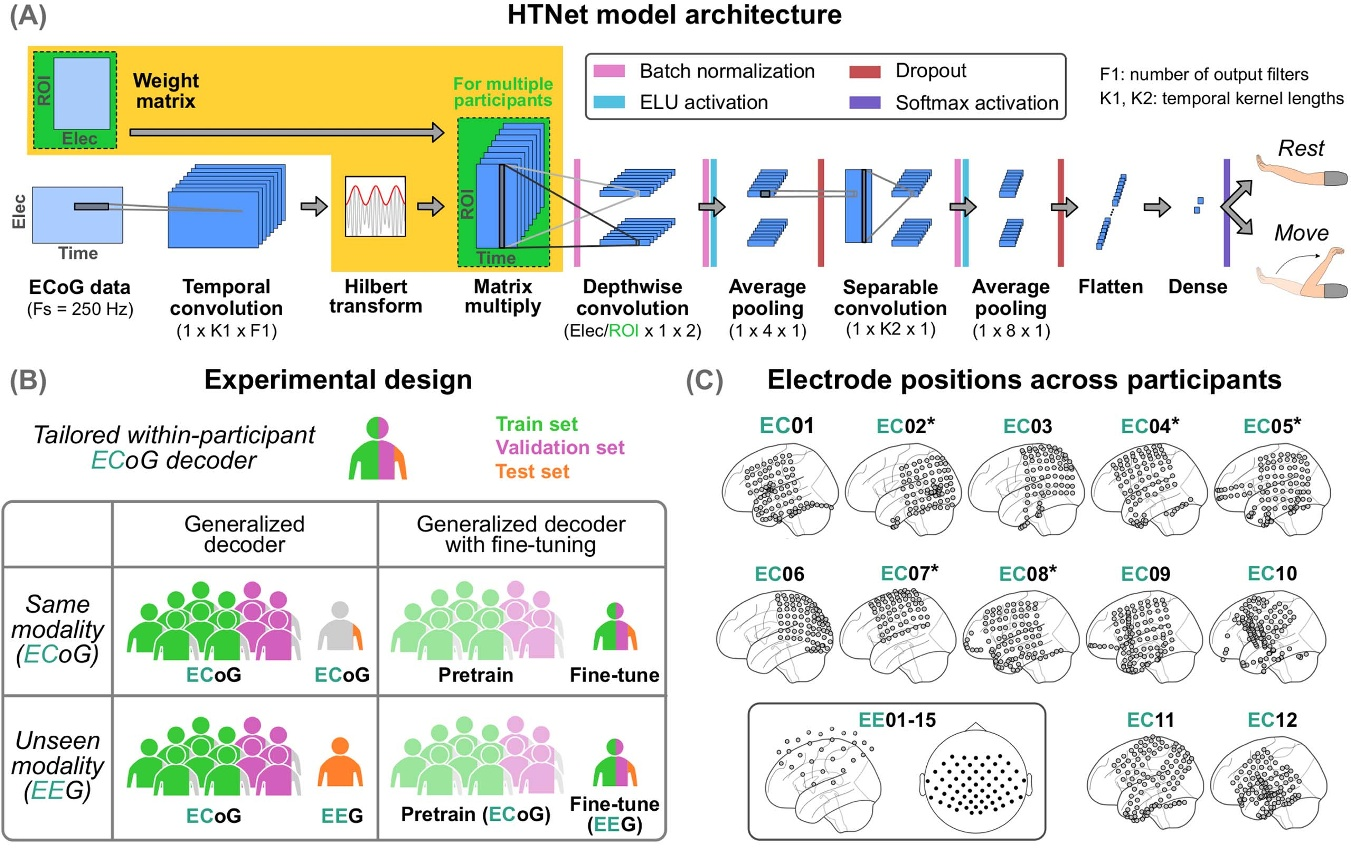
\includegraphics[width=0.8\textwidth]{htnet.png}
	\end{figure}

\end{frame}

%----------------------------------------------------------------------------------------------------------
\begin{frame}{Анализ ошибки}
	\begin{figure}
		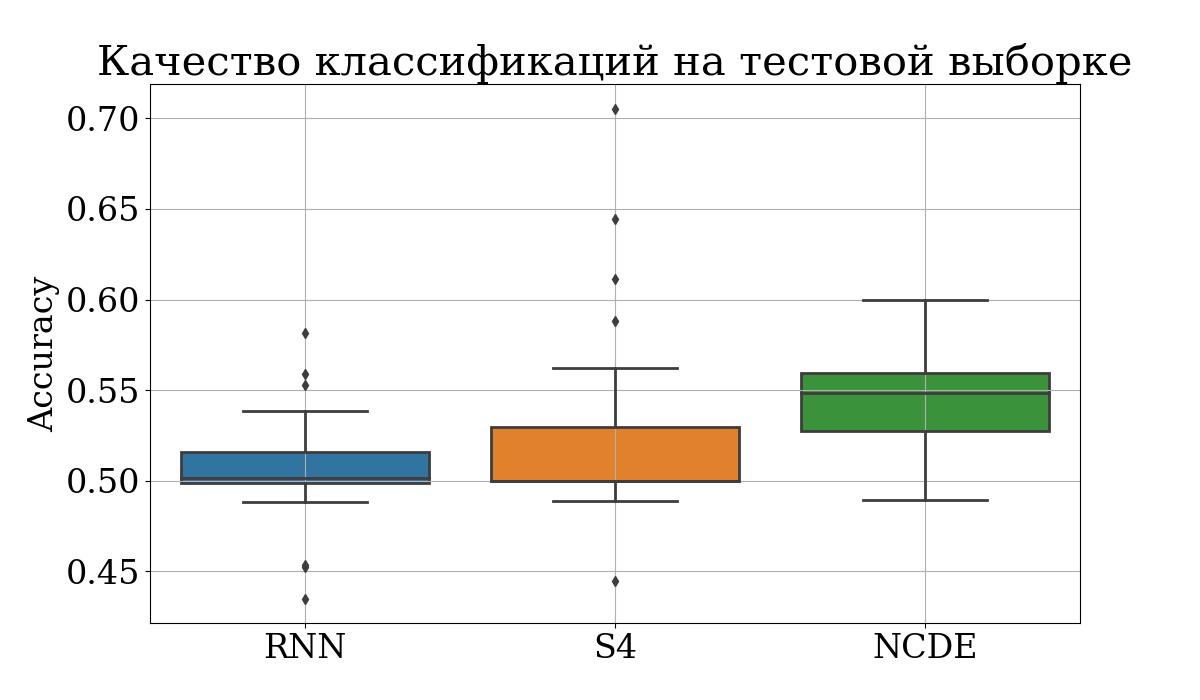
\includegraphics[width=0.5\textwidth]{rnn-s4-ncde.png}
	\end{figure}

	\begin{table}
		\begin{tabular}{c|l|l|l|}
			\cline{2-4}
			\multicolumn{1}{l|}{}  & Parameters & Time per epoch (sec) & Accuracy \\ \hline
			\multicolumn{1}{|c|}{RNN} & 34.2k & 5.86 & 0.506 $\pm$ 0.027 \\ \hline
			\multicolumn{1}{|c|}{S4} & 33.3k & 10.07 & 0.521 $\pm$ 0.049 \\ \hline
			\multicolumn{1}{|c|}{Neural CDE} & 31.5k & 37.23 & 0.546 $\pm$ 0.026 \\ \hline
		\end{tabular}
	\end{table}
\end{frame}

%----------------------------------------------------------------------------------------------------------
\begin{frame}{Заключение}
	\begin{enumerate}
		\item[1] Показано, что рекуррентные нейронные сети, нейронные контролируемые уравнения и модель S4 являются частными случаями модели пространства состояний
		
		\item[2] Продемонстрировано, что NeuralCDE имеет лучшее качество на тестовой выборке по сравнению с другими моделями, однако её время обучения сильно превышает время обучения других моделей
	\end{enumerate}
\end{frame}

\end{document} 